\subsection{Randomizer}
\label{sec:rand}
\begin{description}
	\item[Estimated gates] 1000
	\item[Estimated data bitstream delay] 8 clock cycles for a bit to be
		processed, could be cut to zero by bypassing.
\end{description}

\begin{wrapfigure}{r}{0.5\textwidth}
\begin{center}
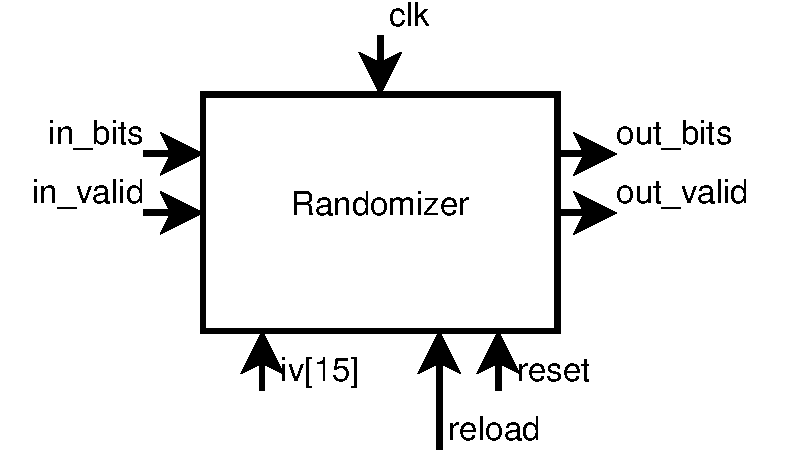
\includegraphics[width=0.48\textwidth]{rand}
\caption{randomizer block diagram}
\label{fig:rand-block}
\end{center}
\end{wrapfigure}

The randomizer operates as a shift register with an initial value
determined by the PDU (packet data unit, one half of a frame) header
and whether it is a UL (uplink) or DL (downlink) PDU.

Internally, the randomizer is implemented as a shift register with a single feedback. 
\autoref{tbl:rand-io} describes the inputs and outputs of the
randomizer. \autoref{fig:rand-block} shows the block representation of the randomizer.

\begin{table*} \begin{tabularx}{\linewidth}{c|c|c|X}
	\label{tbl:rand-io}
	Name & Width & Direction & Description \\ \hline
	
	\wire{reset}     & 1  & I & Resets all internal state
	immediately. The internal register is loaded from
	\wire{iv}. Active low. \\

	\wire{clk}       & 1  & I & Clock. \\

	\wire{in\_bits}  & 1  & I & Uncoded input bitstream to the
	randomizer (this is the first step in the encoding process).\\

	\wire{in\_valid} & 1  & I & Indicates the input bitstream
	\wire{in\_bits} is valid and should be read. \\

	\wire{out\_bits} & 1  & O & Output bitstream. \\
	
	\wire{out\_valid} & 1  & O & Indicates the output bitstream
	is valid. \\

	\wire{iv}        & 15 & I & Initialization data for the
	internal register. \\

	\wire{reload}    & 1  & I & Indicates the internal
	register should be loaded with \wire{iv}. \\

\end{tabularx}
\caption{Randomizer interface definition.}
\end{table*}